\section{Laws with instances}\label{sec:laws}

Each of the seven entries in this section has a general statement and a concrete system in which
its hard hypothesis is proved, in the text below. Hypotheses are labelled (H1), (H2), \dots\ within
each entry.

\subsection{G3: \lawGThree}\label{sec:G3}

\emph{Name.} A potential acts as a \emph{currency}: credit stored in the state pays for expensive
steps later.

Let $s_0 \to s_1 \to \cdots \to s_n$ be a finite stretch of a run in which step $i$ has cost
$a_i$, and let $\Phi \ge 0$ be a potential on states. The \emph{amortized cost} of step $i$ is
$\widehat a_i = a_i + \Phi(s_i) - \Phi(s_{i-1})$.

\begin{theorem}[Amortized potential]\label{thm:G3}
For every finite stretch,
\[
  \sum_{i=1}^{n} a_i \;=\; \sum_{i=1}^{n} \widehat a_i + \Phi(s_0) - \Phi(s_n)
  \;\le\; \sum_{i=1}^{n} \widehat a_i + \Phi(s_0).
\]
If \textup{(H1)} $\widehat a_i \le B$ at every step, then $\sum_{i=1}^n a_i \le nB + \Phi(s_0)$.
\end{theorem}

\begin{proof}
The potential terms in $\sum \widehat a_i$ telescope, and $\Phi(s_n) \ge 0$.
\end{proof}

This is the potential method of amortized analysis \citep{Tarjan1985,CormenEtAl}. G3 is a safety
statement about every finite stretch and says nothing about eventual success; it assumes the
potential rather than constructing it. A potential counts as a certificate only when it is
nonnegative, enters through the exact telescoping formula, and bounds the cost claim actually made.
A statistic that merely correlates with cost does not.

\begin{example}[Binary counter]\label{ex:G3-counter}
Let the state be a binary counter, let an increment cost the number of bits it changes, and let
$\Phi$ be the number of $1$ bits. An increment that turns $r$ trailing ones into zeros and one zero
into a one costs $r + 1$ and changes $\Phi$ by $1 - r$, so its amortized cost is exactly $2$ and
\textup{(H1)} holds with $B = 2$. Hence $n$ increments from zero change at most $2n$ bits, counting a
newly created leading bit as a changed bit.
\end{example}

\Cref{fig:counter} shows the first eight increments.

\begin{figure}[htbp]
\centering
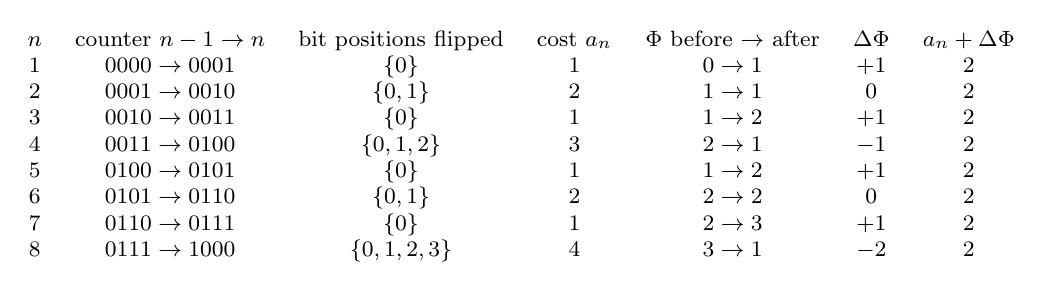
\begin{tikzpicture}
  \node[inner sep=0pt] {\footnotesize
    \begin{tabular}{@{}c c c c c c c@{}}
      \toprule
      $n$ & counter $n-1\to n$ & bit positions flipped & cost $a_n$ & $\Phi$ before $\to$ after & $\Delta\Phi$ & $a_n+\Delta\Phi$ \\
      \midrule
      $1$ & $0000\to0001$ & $\{0\}$       & $1$ & $0\to1$ & $+1$ & $2$ \\
      $2$ & $0001\to0010$ & $\{0,1\}$     & $2$ & $1\to1$ & $0$  & $2$ \\
      $3$ & $0010\to0011$ & $\{0\}$       & $1$ & $1\to2$ & $+1$ & $2$ \\
      $4$ & $0011\to0100$ & $\{0,1,2\}$   & $3$ & $2\to1$ & $-1$ & $2$ \\
      $5$ & $0100\to0101$ & $\{0\}$       & $1$ & $1\to2$ & $+1$ & $2$ \\
      $6$ & $0101\to0110$ & $\{0,1\}$     & $2$ & $2\to2$ & $0$  & $2$ \\
      $7$ & $0110\to0111$ & $\{0\}$       & $1$ & $2\to3$ & $+1$ & $2$ \\
      $8$ & $0111\to1000$ & $\{0,1,2,3\}$ & $4$ & $3\to1$ & $-2$ & $2$ \\
      \bottomrule
    \end{tabular}};
\end{tikzpicture}
\caption{Eight increments from zero, with bit positions numbered from the least significant bit. The displayed potential is the number of $1$ bits.}
\label{fig:counter}
\end{figure}


For a doubling array with $\Phi = \max(0, 2\,\mathrm{size} - \mathrm{capacity})$, every insertion
has amortized cost at most $3$ by the same kind of computation \citep{CormenEtAl}.

\subsection{G4: \lawGFour}\label{sec:G4}

\emph{Name.} The cover of the target family must \emph{move}: which patch covers a target depends
on the target.

Let $\{P(t) : t \in \mathcal T\}$ be an infinite family of targets. A \emph{patch} $\alpha$ comes
with a region $R_\alpha \subseteq \mathcal T$ on which it claims to prove $P$.

\begin{theorem}[Moving-cover exhaustion]\label{thm:G4}
Consider the hypotheses
\begin{itemize}
  \item \textup{(H1)} every patch proves $P(t)$ for every $t$ in its region;
  \item \textup{(H2)} every target lies in the region of some patch;
  \item \textup{(H3)} if $P$ holds everywhere, the declared patches cover every target;
  \item \textup{(H4)} for a declared restricted class of patches, every finite list from the class
    misses some target.
\end{itemize}
Then: (H1) and (H2) give $P(t)$ for every $t$; under (H1) and (H3), $P$ holds everywhere exactly
when the patches cover every target; and under (H4) no finite list from the restricted class covers
every target.
\end{theorem}

\begin{proof}
The first claim applies (H1) to the covering patch. The forward direction of the second is (H3),
and its converse is the first claim. The third is (H4) applied to the given list.
\end{proof}

Each conclusion is close to its hypothesis: (H2) is total coverage, and (H4) already says that every
finite list misses a target. The substance lies in establishing (H2) and (H4) for a system, usually
by a residual for each target that shrinks as the cover grows.

\begin{example}[Initial intervals]\label{ex:G4-intervals}
Let $\mathcal T = \mathbb{N}$, and let the patch with index $a$ cover the interval $[0, a)$. For a
target $t$ the residual $\max(0, t + 1 - a)$ decreases strictly as $a$ grows while it is positive,
and vanishes at $a = t + 1$, so (H2) holds. A finite list of patches misses the largest of its
endpoints, so (H4) holds for the class of all patches. Initial intervals therefore exhaust the
natural numbers as their endpoints grow, although no finite collection of them covers every natural
number.
\end{example}

The greedy expansion of a fraction $p/q \in (0,1)$ into distinct unit fractions is the classical
instance. With $m = \lceil q/p \rceil$ the remainder after subtracting $1/m$ is $(pm - q)/(qm)$,
and $0 \le pm - q < p$, so the numerator strictly decreases and the expansion ends
\citep{Sylvester1880}. A fixed finite set of denominators has finitely many subset sums, so no fixed
package covers all targets; the greedy cover succeeds because its denominators depend on the
target. For the Erd\H{o}s--Straus conjecture ($4/n = 1/x + 1/y + 1/z$ for all $n \ge 2$), a
solution for a prime yields one for its multiples, and no finite family of polynomial identities can
cover the class $n \equiv 1$ modulo every prime because $1$ is a quadratic residue
\citep{Mordell1969}. The conjecture is open, and density results
\citep{Vaughan1970,ElsholtzTao2013} do not give it.

\subsection{G5: \lawGFive}\label{sec:G5}

\emph{Name.} Predicting digit dynamics can need digits from ever deeper positions, as a carry
travels; the \emph{horizon} of useful digits recedes. A closed family of states \emph{confines} the
run when prediction fails.

Let $R : X \to X$ be an update and let a set of \emph{targets} be declared; for reverse-and-add the
targets are the palindromes.

\begin{theorem}[Confinement by a closed pattern]\label{thm:G5}
Let $\mathcal P \subseteq X$ satisfy \textup{(H1)} $R(\mathcal P) \subseteq \mathcal P$ and
\textup{(H2)} no element of $\mathcal P$ is a target. If $R^N(x) \in \mathcal P$, then
$R^{N+t}(x) \in \mathcal P$ and $R^{N+t}(x)$ is not a target for every $t \ge 0$.
\end{theorem}

\begin{proof}
Induction on $t$.
\end{proof}

\subsubsection*{The instance: reverse-and-add in base 2}\label{sec:reverse-add}

A \emph{binary word} here is a word over $\{0,1\}$ that begins with $1$; every positive integer has
exactly one. For a word $w$ let $\bar w$ be its reversal, which may begin with zeros. Binary
reverse-and-add sends $w$ to the binary word of $w + \bar w$, reading both as numbers; we write
$R$ for this map on words and on the positive integers they represent. A word is a
\emph{palindrome} when it equals its reversal. For $r \ge 2$ define the four words
\[
\begin{aligned}
  P_0(r) &= 10\,1^r\,01\,0^r, &\qquad
  P_1(r) &= 11\,0^{r-2}\,1\,000\,1^{r-2}\,01, \\
  P_2(r) &= 10\,1^r\,01\,0^{r+1}, &
  P_3(r) &= 11\,0^r\,10\,1^{r-1}\,01,
\end{aligned}
\]
where $b^j$ denotes $j$ copies of the digit $b$.

\begin{theorem}[Four-phase family]\label{thm:four-phase}
For every $r \ge 2$, as binary words,
\[
  R(P_0(r)) = P_1(r), \qquad R(P_1(r)) = P_2(r), \qquad R(P_2(r)) = P_3(r), \qquad
  R(P_3(r)) = P_0(r+1),
\]
and none of the four words is a palindrome.
\end{theorem}

\begin{proof}
Put $x = 2^r$. The value of each word and of its reversal is a polynomial in $x$ with integer
coefficients, given in \Cref{tab:four-phase}. In each row the value and the reversal add up to the
value of the next word; for the last row, $P_0(r+1)$ has value $12(2x)^2 - 3(2x) = 48x^2 - 6x$.
Since a binary word is determined by its value, each identity of values is an identity of words.
Finally, $P_0$ and $P_2$ begin with $1$ and end with $0$, and $P_1$ and $P_3$ begin with $11$ and
end with $01$, so none equals its reversal.
\end{proof}

\begin{table}[htbp]
\centering
\small
\caption{Values of the four phases and their reversals, with $x = 2^r$.}\label{tab:four-phase}
\begin{tabular}{@{}lllll@{}}
\toprule
Word & Value & Reversal & Sum & Next word \\
\midrule
$P_0(r)$ & $12x^2 - 3x$ & $12x - 3$ & $12x^2 + 9x - 3$ & $P_1(r)$ \\
$P_1(r)$ & $12x^2 + 9x - 3$ & $12x^2 - 15x + 3$ & $24x^2 - 6x$ & $P_2(r)$ \\
$P_2(r)$ & $24x^2 - 6x$ & $12x - 3$ & $24x^2 + 6x - 3$ & $P_3(r)$ \\
$P_3(r)$ & $24x^2 + 6x - 3$ & $24x^2 - 12x + 3$ & $48x^2 - 6x$ & $P_0(r+1)$ \\
\bottomrule
\end{tabular}
\end{table}

The family is recorded in the OEIS and on MathPages \citep{OEIS-A060382,Brown-MathPages}; the proof
here is self-contained.

\begin{corollary}[The orbit of $22$]\label{cor:orbit-22}
The orbit of $22$ under binary reverse-and-add begins
\[
  10110 \;\to\; 100011 \;\to\; 1010100 \;\to\; 1101001 \;\to\; 10110100 = P_0(2),
\]
thereafter runs through $P_1(2), P_2(2), P_3(2), P_0(3), \ldots$, and never reaches a palindrome.
\end{corollary}

\begin{proof}
The first four steps are direct computations ($22 + 13 = 35$, $35 + 49 = 84$, $84 + 21 = 105$,
$105 + 75 = 180$), and none of the four initial words is a palindrome. From $P_0(2)$ on, the family
of \Cref{thm:four-phase} satisfies (H1) and (H2) of \Cref{thm:G5}, so no later word is a
palindrome.
\end{proof}

In base $10$ no such certificate is known: whether the orbit of $196$ reaches a palindrome is
open, and finite searches are evidence only \citep{Walker-Fourmilab}.

\subsubsection*{Why a certificate of this kind is needed}

Let $q_m$ be a family of quotients --- for reverse-and-add in base $b$, $q_m(n) = n \bmod b^m$
records the last $m$ digits --- and let $r_j$ be a family of future readouts, such as the last
digits after $j$ steps.

\begin{schema}[No fixed prediction depth]\label{thm:G5-nogo}
Assume
\begin{itemize}
  \item \textup{(H3)} for every depth $m$ there are a step $j$ and states $y, z$ with
    $q_m(y) = q_m(z)$ and $r_j(y) \ne r_j(z)$.
\end{itemize}
Then no depth $m$ is future-sufficient for the declared readouts.
\end{schema}

\begin{proof}
The pair $y, z$ at depth $m$ is a split pair for $q_m$.
\end{proof}

The template holds for any quotients and readouts. For the Collatz exponent, with
$q_m(n) = n \bmod 2^m$ and the readout $a(n)$, (H3) is \Cref{thm:split-pair}. Whether (H3) holds
for base-$2$ reverse-and-add with a stated family of readouts is open; the confinement of $22$ does
not need it.

\subsection{G8: \lawGEight}\label{sec:G8}\label{sec:abelian}

\emph{Name.} The \emph{odometer} is the vector of firing counts; \emph{abelianization} means that
the order of commuting moves stops mattering.

\begin{definition}[Move system]\label{def:move-system}
A \emph{move system} consists of a set $C$ of configurations, a set $V$ of sites, and for each
$v \in V$ a move $m_v : C \to C$ with a legality predicate $L_v$ on $C$. A \emph{legal run} from $x$
is a finite sequence of sites $v_0, \ldots, v_{\ell-1}$ with $L_{v_i}$ holding at the configuration
reached before step $i$. Its \emph{counter vector} records how often each site occurs. A
configuration is \emph{stable} when no move is legal there.
\end{definition}

\begin{definition}[Abelian compatibility]\label{def:abelian}
The move system satisfies \textup{(H1)} when for every configuration $c$ and all \emph{distinct}
sites $v \ne w$ that are both legal at $c$: $w$ is legal at $m_v(c)$, $v$ is legal at $m_w(c)$,
and $m_w(m_v(c)) = m_v(m_w(c))$.
\end{definition}

\begin{theorem}[Order independence]\label{thm:G8}
Assume \textup{(H1)} and \textup{(H2)}: no infinite sequence of legal moves starts at $x$. If two
legal runs from $x$ end in stable configurations, then they end in the same configuration and have
the same counter vector.
\end{theorem}

\begin{proof}
Induction on the length of the first run. If it is empty, $x$ is stable and the second run is empty
as well. Otherwise let $v$ be its first site. The second run ends in a stable configuration, so $v$
is not legal at its end. By (H1), firing any site other than $v$ keeps $v$ legal, so $v$ occurs in
the second run. Moving that occurrence step by step to the front uses (H1) at each swap, keeps the
run legal, and changes neither its final configuration nor its counter vector. Both runs now begin
with $v$, and the induction hypothesis applies to their remainders from $m_v(x)$.
\end{proof}

This is the abstract form of Dhar's abelian property for sandpiles \citep{Dhar1990}. Under (H2)
every maximal legal run from $x$ is finite and ends in a stable configuration, so all of them end in
one configuration $x^\circ$ with one counter vector $u_x$, the \emph{odometer}.

\begin{example}[Sandpiles]\label{ex:G8-sandpile}
Let $G$ be a finite connected graph with a distinguished sink $s$. A configuration assigns a number
of chips $\eta(v) \ge 0$ to each $v \ne s$. A site $v$ is legal when $\eta(v) \ge \deg(v)$, and
toppling it sends one chip along each edge at $v$; chips sent to $s$ are lost. For distinct legal
$v, w$, toppling $v$ does not decrease $\eta(w)$, so $w$ stays legal, and both orders subtract the
same vector of chip changes; this is (H1). For (H2), suppose an infinite legal run exists. The
number of chips never increases, so every $\eta(v)$ stays bounded. A site that topples infinitely
often sends infinitely many chips to each neighbour, which must then topple infinitely often too.
By connectedness some neighbour of $s$ topples infinitely often, and each such toppling loses a chip
to $s$; this contradicts the finiteness of the chip count. \Cref{thm:G8} therefore gives every
sandpile a unique stable configuration and odometer.

One small case in which sites exchange chips has three mutually adjacent sites, each also
joined to the sink, so that every degree is $3$. Toppling a site removes three of its chips and adds
one to each other site, and one chip is lost to the sink; so every toppling lowers the total by
exactly one, which gives (H2) at once.
\end{example}

\Cref{fig:sandpile} shows one toppling in this case.

\begin{figure}[htbp]
\centering
\begin{tikzpicture}[>=Stealth, site/.style={circle,draw,fill=white,minimum size=8mm,inner sep=0pt,font=\small}]
  \begin{scope}
    \coordinate (a) at (0,1.65);
    \coordinate (b) at (-1.55,-0.85);
    \coordinate (c) at (1.55,-0.85);
    \coordinate (s) at (0,-0.05);
    \draw[gray] (a)--(b)--(c)--(a) (a)--(s) (b)--(s) (c)--(s);
    \draw[->,line width=0.7pt,shorten <=12pt,shorten >=12pt] (a)--(b);
    \draw[->,line width=0.7pt,shorten <=12pt,shorten >=12pt] (a)--(c);
    \draw[->,line width=0.7pt,shorten <=12pt,shorten >=12pt] (a)--(s);
    \node[site,fill=gray!25] at (a) {3};
    \node[site] at (b) {0};
    \node[site] at (c) {0};
    \node[site,fill=gray!12] at (s) {$s$};
    \node[font=\footnotesize,above=15pt] at (a) {$v_1$};
    \node[font=\footnotesize,below left=13pt] at (b) {$v_2$};
    \node[font=\footnotesize,below right=13pt] at (c) {$v_3$};
    \node[font=\small] at (0,3) {before};
  \end{scope}
  \draw[->,line width=0.7pt] (2.3,0.35)--(3.5,0.35)
    node[midway,above,font=\footnotesize] {topple $v_1$};
  \begin{scope}[xshift=5.8cm]
    \coordinate (aa) at (0,1.65);
    \coordinate (bb) at (-1.55,-0.85);
    \coordinate (cc) at (1.55,-0.85);
    \coordinate (ss) at (0,-0.05);
    \draw[gray] (aa)--(bb)--(cc)--(aa) (aa)--(ss) (bb)--(ss) (cc)--(ss);
    \node[site] at (aa) {0};
    \node[site,fill=gray!12] at (bb) {1};
    \node[site,fill=gray!12] at (cc) {1};
    \node[site,fill=gray!12] at (ss) {$s$};
    \node[font=\footnotesize,above=15pt] at (aa) {$v_1$};
    \node[font=\footnotesize,below left=13pt] at (bb) {$v_2$};
    \node[font=\footnotesize,below right=13pt] at (cc) {$v_3$};
    \node[font=\small] at (0,3) {after};
  \end{scope}
\end{tikzpicture}
\caption{One toppling on the three-site graph: $(3,0,0)\to(0,1,1)$. The arrows show one chip sent along each edge from $v_1$, including the edge to the sink $s$.}
\label{fig:sandpile}
\end{figure}


Rotor-routing belongs to the same family of abelian networks \citep{HolroydEtAl2008}. The next two
examples separate the theorem from weaker properties of rewriting systems.

\begin{example}[A unique final configuration without canonical counts]\label{ex:G8-b}
Take configurations $S, A, B, N$ and legal moves $r : S \to A$, $s : S \to B$, $p : A \to N$,
$t : A \to N$, $q : B \to N$, and no others. Every run terminates, and every maximal run ends at $N$.
The three maximal runs $rp$, $rt$ and $sq$ have three different counter vectors. (H1) fails at
$S$: after $r$ the move $s$ is no longer legal.
\end{example}

\begin{example}[Termination without a unique final configuration]\label{ex:G8-d}
Take configurations $S, A, B$ and legal moves $r : S \to A$ and $s : S \to B$ only. Both runs
terminate, at the distinct stable configurations $A$ and $B$.
\end{example}

\begin{remark}[Least action]\label{rem:least-action}
The least-action principle of \citet{FeyLevinePeres2010} compares the odometer with every
nonnegative script of firings that stabilizes the configuration, including scripts that pass
through illegal intermediate configurations. It is imported. The weaker comparison with scripts
that are themselves realized by legal stabilizing runs adds nothing under the hypotheses of
\Cref{thm:G8}, which make all such scripts equal.
\end{remark}

\subsection{G10: \lawGTen}\label{sec:G10}

\emph{Name.} A boundary relation \emph{persists} through a map that is \emph{lossful}, that is,
not injective.

Let $D : X \to X$ be a map, $b : X \to B$ a boundary readout, $\rho : B \to B$ a boundary update, and
$I$ a predicate on $X$, the interior invariant. The run is $x_{n+1} = D(x_n)$.

\begin{theorem}[Persistence through iterated loss]\label{thm:G10}
Assume
\begin{itemize}
  \item \textup{(H1)} $I(x)$ implies $b(D(x)) = \rho(b(x))$, and
  \item \textup{(H2)} $I(x)$ implies $I(D(x))$,
\end{itemize}
and $I(x_0)$. Then $I(x_n)$ and $b(x_n) = \rho^n(b(x_0))$ for every $n \ge 0$.
\end{theorem}

\begin{proof}
Induction on $n$.
\end{proof}

The theorem holds for every map $D$. It is of interest when $D$ is not injective, so that interior
information is lost while the boundary relationship survives because the invariant is regenerated
at every step.

\begin{example}[Checksum cascade]\label{ex:G10-checksum}
On $X = \{0,1\}^2 \times \{0,1\}$ let $D((a, b), c) = ((c, 0), c)$, with boundary $b((a,b),c) = c$,
$\rho$ the identity and invariant $c = a \oplus b$. The map is not injective, and (H1) and (H2)
hold: if $c = a \oplus b$ then the new state $((c, 0), c)$ satisfies $c = c \oplus 0$. The checksum
therefore persists forever while the two data bits are lost.
\end{example}

\subsubsection*{A collapse example: Ducci maps}\label{sec:ducci}

For $n \ge 1$ let $D$ act on cyclic binary vectors $x = (x_0, \ldots, x_{n-1}) \in
\mathbb{F}_2^{\,n}$ by $D(x)_i = x_i + x_{i+1}$, indices modulo $n$.

\begin{theorem}[Ducci nilpotency over $\mathbb{F}_2$]\label{thm:ducci}
If $n = 2^k$, then $D^{\,n}(x) = 0$ for every $x \in \mathbb{F}_2^{\,n}$.
\end{theorem}

\begin{proof}
Write $D = I + S$ with $S$ the cyclic shift. Over $\mathbb{F}_2$, induction on $j$ gives
$D^{2^j}(x)_i = x_i + x_{i+2^j}$, since squaring $I + S^{2^j}$ gives $I + S^{2^{j+1}}$. For $j = k$
the shift $S^{2^k} = S^n$ is the identity, so $D^n(x)_i = 2x_i = 0$.
\end{proof}

The result is classical \citep{ChamberlandThomas2004,Breuer2007b}. For vectors of length $2^k$ the
parity structure is destroyed completely, so no nonzero persistence claim for all such vectors can
rest on parity.

\begin{remark}[Integer Ducci tuples]\label{rem:ducci-integer}
The integer Ducci map sends $(x_0, \ldots, x_{n-1})$ to $(|x_0 - x_1|, \ldots, |x_{n-1} - x_0|)$.
Modulo $2$ it is $D$, and it commutes with multiplication by $2$. For $n = 2^k$, \Cref{thm:ducci}
makes every entry even after $n$ steps, after which the run is twice another Ducci run. Since the
entries never exceed the largest entry of the first iterate, they become divisible by arbitrarily
large powers of $2$ and hence vanish. For $n = 4$ the argument gives an explicit bound: every
$x \in \mathbb{N}^4$ reaches the zero tuple after $4m$ steps of the integer map, where $m$ is the
largest entry of $x$, because after
$4k$ steps every entry is a multiple of $2^k$ and at most $m$, and $2^m > m$. For other lengths
integer tuples can cycle without reaching zero, for example $(0,1,1) \to (1,0,1) \to (1,1,0) \to
(0,1,1)$.
\end{remark}

Gilbreath's conjecture, read as a persistence claim for the leading entry of iterated absolute
differences of the primes, is open \citep{Odlyzko1993}.

\subsection{G12: \lawGTwelve}\label{sec:G12}

\emph{Name.} A finite witness \emph{radiates}: its images under the symmetries of the graph are
witnesses too.

Let $E$ be a graph relation on a set $X$. A \emph{proper $k$-colouring} is a map $c : X \to \{1,
\ldots, k\}$ with $c(x) \ne c(y)$ whenever $E(x, y)$. A \emph{finite witness} for $k$ is a finite set
$W \subseteq X$ whose induced graph has no proper $k$-colouring. A map $\gamma : X \to X$
\emph{preserves} $E$ when $E(x, y) \Leftrightarrow E(\gamma x, \gamma y)$.

\begin{theorem}[Finite witnesses]\label{thm:G12}
Let $W$ be a finite witness for $k$.
\begin{enumerate}
  \item $X$ has no proper $k$-colouring.
  \item If $\gamma$ preserves $E$, then $\gamma(W)$ is a finite witness for $k$.
\end{enumerate}
\end{theorem}

\begin{proof}
A proper colouring of $X$ restricts to one of $W$. A proper colouring $c$ of $\gamma(W)$ pulls back
to the proper colouring $c \circ \gamma$ of $W$, because $\gamma$ sends edges to edges; $\gamma$
need not be injective.
\end{proof}

\begin{example}[The Moser spindle]\label{ex:G12-moser}
In the plane with $E(x, y)$ meaning $\lVert x - y \rVert = 1$, take two rhombi with vertices $A, B, D, C$ and
$A, B', D', C'$ in cyclic order and unit sides, each made of two equilateral unit triangles ($ABC$,
$BCD$ and $AB'C'$, $B'C'D'$), so that $A$ and $D$ are opposite vertices with
$\lVert A - D \rVert = \sqrt 3$, and likewise $\lVert A - D' \rVert = \sqrt 3$. Rotate the second
rhombus about $A$ by the angle $\theta$ with $2\sqrt 3 \sin(\theta/2) = 1$, which exists because
$1 < 2\sqrt 3$; then $\lVert D - D' \rVert = 1$. The seven points $A, B, C, D, B', C', D'$ are
distinct, and the eleven pairs $AB, AC, BC, BD, CD$, $AB', AC', B'C', B'D', C'D'$ and $DD'$ are at
unit distance. In a proper
$3$-colouring, $B$ and $C$ take the two colours other than that of $A$, so $D$ takes the colour of
$A$; likewise $D'$ does, and $D, D'$ are adjacent. So the seven points form a finite witness for
$k = 3$, and $\chi(\mathbb{R}^2) \ge 4$ by \Cref{thm:G12}; by part~2, so does every rotated and
translated copy.
\end{example}

\Cref{fig:moser} shows the seven points and the eleven unit distances.

\begin{figure}[htbp]
\centering
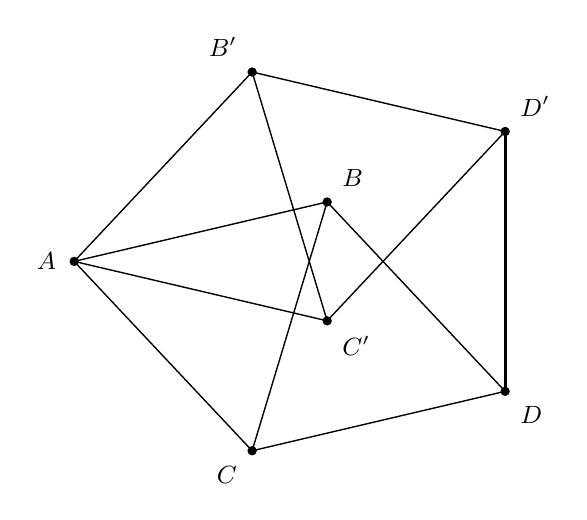
\begin{tikzpicture}[scale=3.3, every node/.style={font=\small}]
  % The long diagonals AD and AD' have length sqrt(3). Their angles are
  % -alpha and +alpha, where alpha = asin(1/(2 sqrt(3))).
  \coordinate (A)  at (0,0);
  \coordinate (B)  at (0.973493765,0.228713554);
  \coordinate (C)  at (0.684818630,-0.728713554);
  \coordinate (D)  at (1.658312395,-0.500000000);
  \coordinate (Bp) at (0.684818630,0.728713554);
  \coordinate (Cp) at (0.973493765,-0.228713554);
  \coordinate (Dp) at (1.658312395,0.500000000);
  \draw[line width=0.5pt] (A)--(B)--(D)--(C)--cycle;
  \draw[line width=0.5pt] (B)--(C);
  \draw[line width=0.5pt] (A)--(Bp)--(Dp)--(Cp)--cycle;
  \draw[line width=0.5pt] (Bp)--(Cp);
  \draw[line width=1pt] (D)--(Dp);
  \fill (A) circle (0.018) node[left=3pt] {$A$};
  \fill (B) circle (0.018) node[above right=2pt] {$B$};
  \fill (C) circle (0.018) node[below left=2pt] {$C$};
  \fill (D) circle (0.018) node[below right=2pt] {$D$};
  \fill (Bp) circle (0.018) node[above left=2pt] {$B'$};
  \fill (Cp) circle (0.018) node[below right=2pt] {$C'$};
  \fill (Dp) circle (0.018) node[above right=2pt] {$D'$};
\end{tikzpicture}
\caption{Two unit rhombi sharing $A$, with the second rotated by $\theta$ where $2\sqrt3\sin(\theta/2)=1$. The heavier edge joins $D$ and $D'$; all eleven drawn edges have unit length.}
\label{fig:moser}
\end{figure}


\begin{proposition}[Completeness of finite witnesses under compactness]\label{prop:G12-compact}
Assume
\begin{itemize}
  \item \textup{(H1)} if $X$ has no proper $k$-colouring, then some finite witness for $k$ exists.
\end{itemize}
Then $X$ has no proper $k$-colouring exactly when a finite witness for $k$ exists.
\end{proposition}

\begin{proof}
The forward direction is the hypothesis and the backward direction is \Cref{thm:G12}.
\end{proof}

The hypothesis is the de~Bruijn--Erd\H{o}s theorem \citep{BruijnErdos1951}, which uses the axiom of
choice. For the unit-distance graph of the plane the current bounds are $5 \le \chi(\mathbb{R}^2)
\le 7$. The lower bound is a finite witness in exactly the sense of \Cref{thm:G12}: de~Grey
constructed a $1581$-vertex unit-distance graph that is not $4$-colourable \citep{DeGrey2018}, and
later work reduced this to $553$ vertices \citep{Heule2018} and to $509$ \citep{Parts2020}. The
upper bound is the classical hexagonal colouring. The exact value is open, and questions of this
kind can depend on the set-theoretic background \citep{ShelahSoifer2003,Falconer1981}; the finite
lower bound does not, once the graph and its non-colourability are accepted.

\subsection{G13: \lawGThirteen}\label{sec:G13}

\emph{Name.} An orbit that is \emph{thin} (sparse in a precise sense) can still \emph{saturate} a
target, missing only a vanishing proportion of it.

Let $m, t : \mathbb{N} \to \mathbb{N}$ count, up to $N$, the missed members and all members of a
target set.

\begin{theorem}[Relative density]\label{thm:G13-density}
If $m(N) = o(N)$ and $t(N) \ge cN$ for all $N$ with a fixed $c > 0$, then $m(N) = o(t(N))$.
\end{theorem}

\begin{proof}
Given $\varepsilon > 0$, eventually $m(N) \le \varepsilon c N \le \varepsilon\, t(N)$.
\end{proof}

\begin{example}[Powers of two]\label{ex:G13-powers}
Let the target be the positive integers and let the represented set be the integers that are not
powers of two. The missed family, the powers of two, is infinite, and its count up to $N$ is at most
$\lfloor \log_2 N \rfloor + 1$, so its relative density is zero by \Cref{thm:G13-density} with
$t(N) = N$. The represented set has density one and still misses infinitely many targets.
\end{example}

This is a small arithmetic example of the counting phenomenon, not a thin-orbit result. The setting
that motivates G13 is a group $\Lambda$ acting on a discrete set, with an orbit projected to integers
and observed against a target $A$. There $\Lambda$ is \emph{thin} (Zariski dense of infinite index in
an arithmetic group) and $A$ is \emph{thick} (a finite union of residue classes, so of positive
density).

\begin{schema}[Thin orbits saturate thick targets]\label{thm:G13}
Assume that $\Lambda$ is thin, that its congruence quotients have a uniform spectral gap, that $A$
passes the local congruence conditions, and
\begin{itemize}
  \item \textup{(H1)} an imported theorem gives $m(N) = O(N^{1-\eta})$ for some $\eta > 0$.
\end{itemize}
Then the proportion of missed admissible targets tends to zero.
\end{schema}

\begin{proof}
(H1) gives $m(N) = o(N)$, and a thick target gives $t(N) \ge cN$ for all large $N$, which suffices
for the argument of \Cref{thm:G13-density}. The first three hypotheses are the setting in which such
bounds are proved and are not used.
\end{proof}

Apollonian circle packings are the motivating instance. Curvatures of four mutually tangent circles
satisfy Descartes' relation $k_1^2 + k_2^2 + k_3^2 + k_4^2 = \tfrac12 (k_1 + k_2 + k_3 + k_4)^2$,
and the integral packing generated from $(-1, 2, 2, 3)$ has curvatures only in the residue classes
$\{2, 3, 6, 11, 14, 15, 18, 23\}$ modulo $24$. Bourgain and Fuchs proved that the curvatures have
positive density \citep{BourgainFuchs2010}, and Bourgain and Kontorovich that almost every admissible
integer occurs, with $O(N^{1-\eta})$ exceptions \citep{BourgainKontorovich2014Apollonian}. Haag,
Kertzer, Rickards and Stange showed that the full local-to-global conjecture is nevertheless false
for many packings: certain quadratic and quartic families pass the congruence conditions and are
still missed, for reasons of quadratic reciprocity \citep{HaagEtAl2024}. Those families have density
zero, so they do not contradict the template; they are a second kind of exception, distinct from
failing a congruence condition, and \Cref{ex:G13-powers} is the same pattern in miniature.
